\documentclass[a4paper,12pt]{article}
\usepackage{multirow}
\usepackage{graphicx}
\usepackage[utf8]{inputenc}
\usepackage[english]{babel}
\usepackage{hyperref}
\usepackage{longtable,tabu}
\usepackage{pdflscape}
\usepackage{float}
\usepackage{tabularx}
\usepackage{mathtools}
\usepackage{csquotes}
\usepackage[nottoc,numbib]{tocbibind}
\usepackage[backend=biber,style=ieee,sorting=none]{biblatex}
\usepackage{hyperref}
\usepackage{listings}
\usepackage{color}

\definecolor{dkgreen}{rgb}{0,0.6,0}
\definecolor{gray}{rgb}{0.5,0.5,0.5}
\definecolor{mauve}{rgb}{0.58,0,0.82}

\lstset{frame=tb,
  language=C++,
  aboveskip=3mm,
  belowskip=3mm,
  showstringspaces=false,
  columns=flexible,
  basicstyle={\small\ttfamily},
  numbers=none,
  numberstyle=\tiny\color{gray},
  keywordstyle=\color{blue},
  commentstyle=\color{dkgreen},
  stringstyle=\color{mauve},
  breaklines=true,
  breakatwhitespace=true,
  tabsize=3
}

\addbibresource{report.bib}
\hypersetup{
    colorlinks=true,
    linkcolor=blue,
    filecolor=magenta,
    citecolor=cyan,
    urlcolor=cyan
    }

\begin{document}


\begin{titlepage}
  \centering
  
\includegraphics[width=0.15\textwidth]{iitkgp.png}\par\vspace{1cm}
  {\scshape\LARGE Indian Institute of Technology, Kharagpur \par}
  \vspace{1cm}
  {\scshape\Large Seminar Report \\ on \par}
  \vspace{1.5cm}
  {\huge\bfseries Thread Extraction Strategies \par}
  \vspace{2cm}
  {Prepared by\par\Large\itshape Abhishek Tiwari \textnormal{(16CS60R83)}\par}
  \vfill
  Supervised by\par
  Lec.~Partha Sarathi.~\textsc{Dey}

  \vfill

% Bottom of the page
  {\large \today\par}
\end{titlepage}




\newpage
\tableofcontents
\listoffigures
\newpage

\begin{center} \LARGE \textbf{Abstract} 
\end{center}

Multi Core Processors have come into existence for quite some time now. But currently the true power of Multi Core Processor largely remain unutilized because of non availability of any standard Thread Level Parallelism [TLP] platform . Policies needs to be framed for the task of extraction of concurrently executable threads from a given High Level Code utilizing available libraries (if possible) to be done at the Compilation Stage at the latest. This is to be followed by the Thread allocation to one core among the available cores following some other Thread Allocation/Scheduling policy to be done by the Operating System. This paper proposes some policies for both.
\\
\\
\textbf{Keywords:}
Multicore processors, Thread Extraction, Intel Thread Building Blocks, Thread Isolation, Speculative Multithreaded Processors
\newpage
\section{Introduction}
Ever since the advent of Multi Core Processors, in which several identical processing cores [ Where each core does possess it’s own Instruction Pipeline as well as it’s own ALU, Associated Registers, Flags, General Purpose Register [GPR] files, Special Purpose Registers like Stack Pointers, Instruction Pointer, Segment Registers and exclusively owned Instruction Cache (I-Cache) Data Cache (D-Cache) ] exists within the same CPU, efforts are on to increase the CPU performance in the form of enhance throughput by exploiting Thread Level Parallelism (TLP) in these different cores.
\\
One approach is designing every program based on some form of generic Parallel Algorithm in which the programmer has the major say in isolation of the number of threads which later on will be transformed into several simultaneous executable Assembly code blocks by the underlying compiler . Each of these Assembly code blocks in turn will need to be converted into an executable code block which needs to be scheduled/ allocated to the available Core Pool by the underlying Operating System. This however involves rewriting of most of the existing codes based on some parallel algorithm which may not be always feasible or advisable. 
\\
Another and more acceptable approach happens to be identification and extraction of threads from existing High Level Programs to be performed partly by the programmer aided by some specially developed libraries like Open MP and partly by the underlying Compiler by employing some special algorithms. Once extracted , each of these threads needs to be allocated and scheduled to the available Core Pool adopting some policies by the underlying Operating System.

\section{ Program vs Process vs Thread}
\begin{enumerate}
\item \textbf{Program} is an executable file residing on the disk. It must be loaded into memory in order to begin execution. A program is thus a \textbf{passive} entity.
\\
\textbf{For example:} In Unix based system ls is program that resides in /bin/ls

\item A \textbf{Process} is an executing instance of a program. It is thus an \textbf{active} entity. Processes can be executed in parallel if the operating system supports multiprocessing. The parallel execution of processes is handled by the kernel.
\\
\textbf{For example:} Executing multiple instances of a chat server. Thus whenever a client connects to server, a separate process can be forked at the server in order to process the client requests.

\item A \textbf{Thread} is a lightweight process. It execcutes within the context of a process. A process can be break into multiple threads in order to execute tasks concurrently. The threads of same process share same address space, file descriptor, stack and other process related attributes. A thread however has its private memory too, and its own stack. 
\\
\textbf{For example:} Matrix Multiplication can be performed in parallel by concurrently executing threads.
\end{enumerate}

\section{Motivation for Thread Extraction}
There has been significant advancement in the hardware architecture of the processor which are still not being fully utilized. There are following capabilities of processor that leads to study of thread extraction strategies:
\subsection{Time Sharing and Multi Tasking}
Time Sharing enables the use of system simultaneously by different users. Switching is performed in order to process different user requests. The main objective in such time sharing system is to reduce the response time. 
\\
Multitasking is performing different tasks on a system concurrently. Multiple process are served by doing context switching. This task of scheduling different process is handled by the process scheduler.
\subsection{Multi-Threading and Hyper-Threading}
Muti-Threading enables execution of different threads of a process simultaneouly. These multiple threads can be handled at the user level as well as can be scheduled by the kernel to execute parallely. Usually the threads that execute are independent of each other but \textbf{Speculative Multithreading} enables distribution of a task into multiple threads even if they are not mutually independent.
\\
Hyperthreading (Simultaneous Multi-threading) is a hardware enhancement in order to execute multiple threads simultaneously. This enhancement is done by installing multiple pipelines in the system.
\\
\begin{minipage}{\textwidth}
\textbf{If there are N processors and each processor has M cores then if K threads can be executed per core, then total number of threads that can be executed simultaneouly are:}
\begin{center}
 \Large \textbf{N*M*K}
\end{center}
\end{minipage}
\section{Rationale for Speculative Multithreading}
The motivation for using speculative multithreading comes from two directions. On one hand, the potential for further increasing single-program performance using known parallelism extraction techniques is diminishing. On the other, technology trends suggest processors that can execute multiple threads of code. These circumstances invite us to find those few innovations that will enable such multithreaded processors to support the parallel execution of a single program.\cite{speculative}

\subsection{Limitations of Existing Techniques to Extract Parallelism}
In current scenarios, at runtime a super-scalar processor unrolls the static control flow to produce a dynamic instruction stream. The positions of reader and writer instructions in this stream defines the way data flows from one operation to another, i.e., the algorithm itself. A super-scalar processor creates a dynamic instruction window (an unrolled contiguous segment of the dynamic instruction stream), repeatedly searches this window for unexecuted, independent instructions, and attempts to execute these instructions in parallel. Sustained high-performance demands that any given window contain a sufficient number of independent instructions, i.e., a sufficient level of instruction-level parallelism (ILP).
\\
Instruction Level Parallelism cannot be always achieved. It is limited by the fact that the processor should process the available window of instruction in order to extract independent instructions that can be executed simultaneously. This problem can be solved by taking larger window size but again there would be other programming challenges. Speculative multithreading is such a model to overcome these challenges. In speculative multithreading, each program region is considered to be a speculative thread, i.e., a small program. By executing multiple speculative threads in parallel, additional parallelism can be extracted (especially if each thread is mostly sequential). The threads are subsequently merged to recreate the original program. Speculative multithreading allows a large instruction window to be created as an ensemble of smaller instruction windows, thereby facilitating implementation. In addition, a proper thread division can logically isolate branches in one thread from those in another, relieving the fundamental problem of diminishing instruction utility.
\subsection{The Emergence of Multithreaded Architectures}
Multithreaded processors — processors that support the concurrent execution of multiple threads on a single chip — are beginning to look as if they willdominate the landscape of the next decade. Two multithreaded processor models are currently being explored.\cite{multithreaded}
\begin{enumerate}
\item Simultaneous multithreading (SMT)- uses a monolithic design with most resources shared amongst the threads.

\item Chip multiprocessing (CMP)- proposes a distributed design (a collection of independent processing elements) with less resource sharing.

\end{enumerate}

\newpage

\section{Thread Extraction Policies}
There are following thread extraction policies that can be applied-

\subsection{Programmer Controlled}
\begin{enumerate}
\item Programmer specifies the start and end of threads.
\item Compiler reads markers in order to extract threads and creating thread pool.
\item \textbf{For eg-} Using OpenMP constructs to mark parallel thread execution.
\end{enumerate}
\begin{lstlisting}
/***************************************************************************
* DESCRIPTION:  
*   OpenMp Example - Matrix Multiply - C Version
*   Demonstrates a matrix multiply using OpenMP. Threads share row iterations
*   according to a predefined chunk size.
* AUTHOR: Blaise Barney
* LAST REVISED: 06/28/05
******************************************************************************/
#include <omp.h>
#include <stdio.h>
#include <stdlib.h>

#define NRA 62                 /* number of rows in matrix A */
#define NCA 15                 /* number of columns in matrix A */
#define NCB 7                  /* number of columns in matrix B */

int main (int argc, char *argv[]) 
{
int	tid, nthreads, i, j, k, chunk;
double	a[NRA][NCA],           /* matrix A to be multiplied */
	b[NCA][NCB],           /* matrix B to be multiplied */
	c[NRA][NCB];           /* result matrix C */

chunk = 10;                    /* set loop iteration chunk size */

/*** Spawn a parallel region explicitly scoping all variables ***/
#pragma omp parallel shared(a,b,c,nthreads,chunk) private(tid,i,j,k)
  {
  tid = omp_get_thread_num();
  if (tid == 0)
    {
    nthreads = omp_get_num_threads();
    printf("Starting matrix multiple example with %d threads\n",nthreads);
    printf("Initializing matrices...\n");
    }
  /*** Initialize matrices ***/
  #pragma omp for schedule (static, chunk) 
  for (i=0; i<NRA; i++)
    for (j=0; j<NCA; j++)
      a[i][j]= i+j;
  #pragma omp for schedule (static, chunk)
  for (i=0; i<NCA; i++)
    for (j=0; j<NCB; j++)
      b[i][j]= i*j;
  #pragma omp for schedule (static, chunk)
  for (i=0; i<NRA; i++)
    for (j=0; j<NCB; j++)
      c[i][j]= 0;

  /*** Do matrix multiply sharing iterations on outer loop ***/
  /*** Display who does which iterations for demonstration purposes ***/
  printf("Thread %d starting matrix multiply...\n",tid);
  #pragma omp for schedule (static, chunk)
  for (i=0; i<NRA; i++)    
    {
    printf("Thread=%d did row=%d\n",tid,i);
    for(j=0; j<NCB; j++)       
      for (k=0; k<NCA; k++)
        c[i][j] += a[i][k] * b[k][j];
    }
  }   /*** End of parallel region ***/

/*** Print results ***/
printf("******************************************************\n");
printf("Result Matrix:\n");
for (i=0; i<NRA; i++)
  {
  for (j=0; j<NCB; j++) 
    printf("%6.2f   ", c[i][j]);
  printf("\n"); 
  }
printf("******************************************************\n");
printf ("Done.\n");

}
\end{lstlisting}

\subsection{Compiler Driven}
\begin{enumerate}
\item The Compiler creates the Thread Pool during parsing starting from the Parse Trees.
\item Independent parts of program are executed simultaneously.
\item Compiler cannot always resolve dependencies that can be handled at hardware level.\cite{tls}
\item \textbf{For example:} Intel TBB, which uses speculative thread extraction strategy to parallely run a program.
\end{enumerate}
\textbf{Intel TBB- Dynamic Scheduling of Tasks: }
\\
The TBB runtime library consists of a dynamic scheduler that stores and distributes available parallelism as needed in order to improve performance. While this dynamic management of parallelism is completely hidden from the programmer, it imposes a management “tax” on performance, which at significant levels can be detrimental to parallelism performance.When the TBB runtime library is first initialized, a set of slave worker threads is created and the caller of the initialization function becomes the master worker thread.

\subsection{Architecture Driven}
\begin{enumerate}
\item At hardware level, there is instruction level parallelism.
\item The instructions are rearranged in independent blocks of instruction and executed simultaneously.
\item Speculative parallelism helps to resolve any hazards due to dependency between the blocks of instruction.
\item \textbf{For example:} The threads can be executed in parallely by diving them into further threads at instruction level.
\end{enumerate}
\subsubsection {Dividing Program into Multiple Thread}
There are several ways in which to divide programs into threads. We categorize these divisions as control-driven and data-driven depending on whether threads are divided primarily along control-flow or data-flow boundaries. Each division strategy can be further sub-categorized as either non-speculative the threads are completely independent from the point of view of the processor and any dependence is explicitly enforced using architectural synchronization constructs, or speculative — the threads may not be perfectly independent, or synchronized, and it is up to the hardware to detect and potentially recover from violations of the independence assumptions.

\section{The Case Studies}
\subsection{Performance Measure for Programmed Thread Strategy}
\begin{figure}[H]
  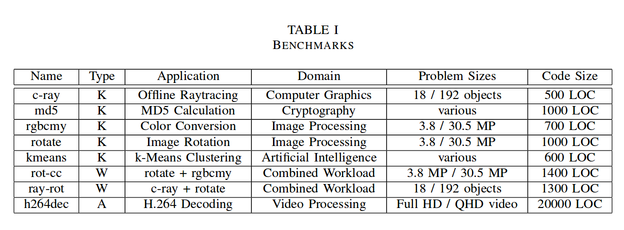
\includegraphics[width=\textwidth,height=10cm]{benchmark.png}
  \caption{The Benchmark Codes (K-Kernel, W-Workload, A-Application, LOC-Lines Of Code)}
  \label{fig:benchmark}
\end{figure}

This table contains various benchmark codes for measuring performance of openmp/SMPSs.
\\ 
\begin{figure}[H]
  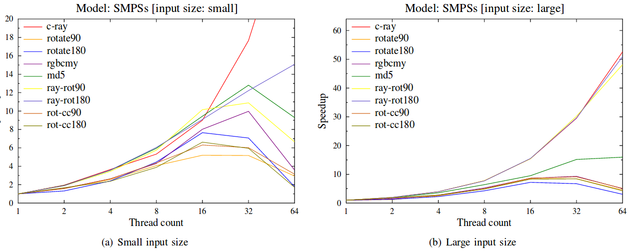
\includegraphics[width=\textwidth,height=10cm]{mpenthreads.png}
  \caption{Baseline Performance For OpenMp/SMPSs }
  \label{fig:openmp}
\end{figure}

The above figure depicts the performance measure of the benchmark codes that are programmed using openmp/SMPS contructs by the programmer. There is relatively higher performance gain for large programs as compared to small ones. The performance gain is also limited by the number independent threads that can be run simultaneously on the system. For example- If the number of threads supported are less than the threads in the program then some threads have to be scheduled on the same core of the processor and cannot be run simultaneouly. Ideal condition is that all the cores are fully utilized and there are that many threads defined in the program.\cite{benchmark}

\subsection{Performance Measure for Architecture Driven/ Compiler Based Strategy}
Here the Intel TBB is applied and performance is measured for various multicore processors that are simulated by Intel TBB.
\begin{figure}[H]
  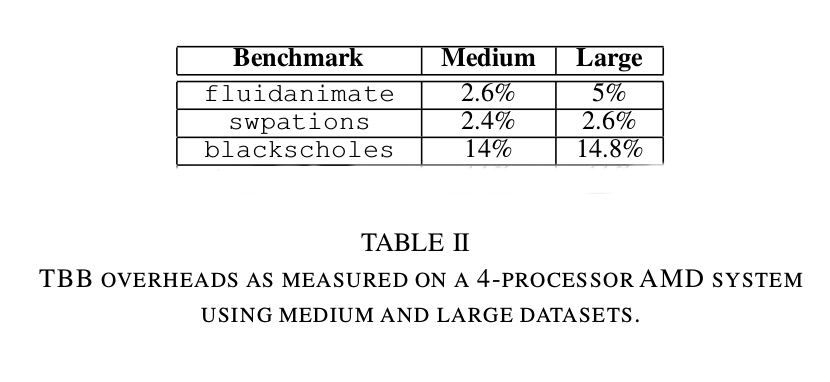
\includegraphics[width=\textwidth,height=10cm]{table2.png}
  \caption{The Benchmark Codes}
  \label{fig:table2}
\end{figure}
For the above benchmark codes, performance of Intel TBB is measured as follows-
\begin{figure}[H]
  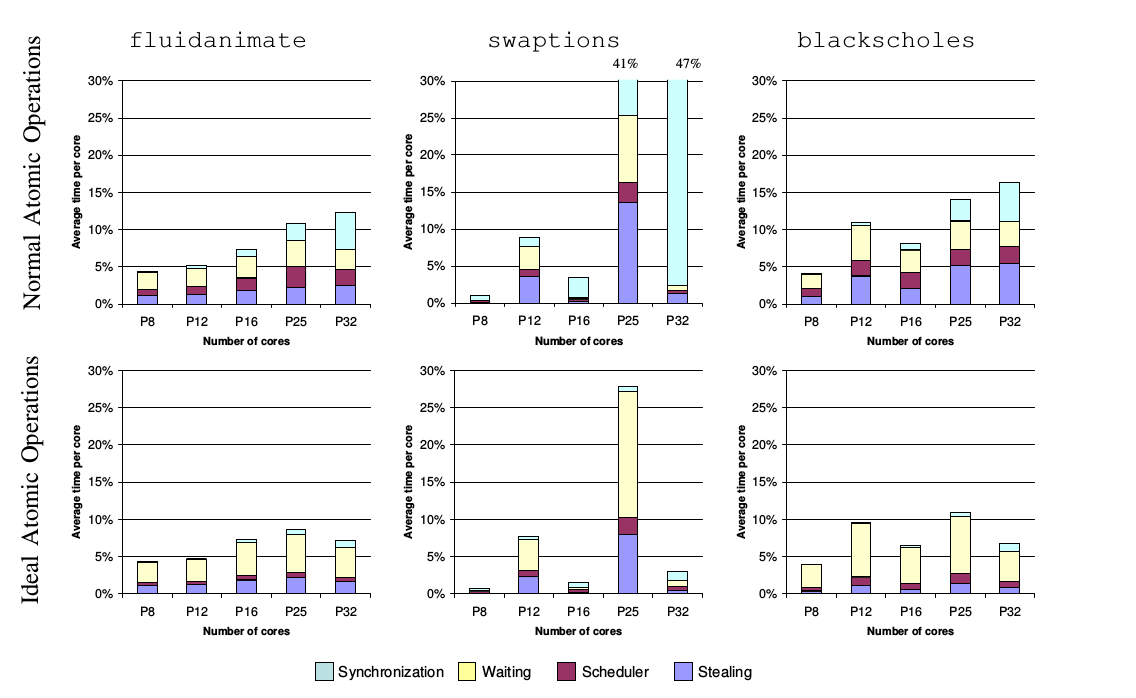
\includegraphics[width=\textwidth,height=10cm]{diag.png}
  \caption{Average contribution per core of the TBB runtime library on three PARSEC benchmarks }
  \label{fig:inteltbb}
\end{figure}

In the above figure TBB contribution is broken down into four categories. The top row shows TBB contribution when latency of atomic operations is appropriately modeled. The bottom row shows TBB contributions when atomic operations are modeled as 1-cycle latency instructions.\cite{inteltbb}

\section{Conclusion}
\begin{enumerate}
\item As there has been significant advancement in hardware, softwares needs to be modified in order to fully exploit the capabilities of the system.
\item Intel TBB encourages to automate the task of running serial tasks in parallel by applying thread level speculation.
\end{enumerate}
There are capabilities of microprocessors that are yet to be exploited so that the softwares are able to utilize the computational power of system efficiently.
\printbibliography[heading=bibintoc]
\end{document}
